% status: 0
% chapter: TBD

\title{Twilio}


\author{Ramyashree DG}

\affiliation{%
  \institution{Indiana University Bloomington}
  \city{Bloomington} 
  \state{Indiana} 
  \postcode{47404}
}
\email{rdasego@iu.edu}

\author{Gregor von Laszewski}
\affiliation{%
  \institution{Indiana University}
  \streetaddress{Smith Research Center}
  \city{Bloomington} 
  \state{IN} 
  \postcode{47408}
  \country{USA}}
\email{laszewski@gmail.com}


% The default list of authors is too long for headers}
\renewcommand{\shortauthors}{G. v. Laszewski}


\begin{abstract}

Twilio is a  developer platform to enable communications between the business 
applications and the customers. The purpose of this paper is to discuss 
regarding Cloud platform to enable communication with the customers. Twilio is 
neither a software application nor a communication system, it lies at the 
intersection of both. Twilio makes communication as user interface element 
rather than being a separate infrastructure. Twilio seeks to rid businesses of 
the messy telecom hardware by providing a telephony infrastructure web service
software-based platform which enables customers to easily add voice, messaging
and video to their apps,  providing developers with the predesigned APIs needed
to build any communication-based functionality which is suitable for the 
business application. Popular use cases include ridesharing apps enabling 
anonymous communication between passengers and drivers and e-commerce companies
sending automated delivery notifications or promotional messages.

\end{abstract}

\keywords{hid-sp18-406, Twilio, Cloud Service, Communication Platform,
Integration API}

\maketitle

\section{Introduction}

Nowadays updating information to communicate between the applications and 
customers is done through the text messages and emails. Communication enables 
the business people to be involved with their customers and on the other hand
to capture the interest of customers which are increasingly sophisticated. 
This process of managing company’s relationships and interactions with the 
customers is called Customer Relationship Management
~\cite{hid-sp18-406-twilio-intro1}. However, maintaining the communication 
implementation from the scratch for every business oriented applications will 
lead to wastage of resources. To enable the business entrepreneurs to focus 
their time on implementing the services required for improving the user 
experiences Twilio provides a common developer platform to design the 
communications to the customers. Using this platform software developers can add
SMS and instant messages, video or voice calling apps without owning the 
back-end infrastructure to maintain the services. This is achieved by providing
developers with APIs which are required to build communication-based 
functionality which best suits their application.  All of these required 
infrastructure is virtualized in the cloud and made available as building 
blocks through Mobile and Web APIs. Therefore, this cloud-based service enables
powerful communication between mobile devices, applications, services, and 
systems throughout the business and helps to build the bridge for the 
communication between the business application and its customers
~\cite{hid-sp18-406-twilio-intro2}. 

\section{Architecture}

The main design principle of Twilio is enabling serverless architecture which is
known as serverless computing or function as a service for the business 
applications. Twilio hosts the server and eliminates the need for developers to 
focus on services which are out of scope for the main business domain. This 
architecture provides the flexibility of enabling functions individually and 
scaling up based on the requirements. Each function required for communication 
integrations is hosted by Twilio as Function as a Service which is called FaaS. 
Typically, all the management such as physical server establishment, deploying 
the operating system, web hosting processes through virtual servers is managed 
by Twilio and provides a final API which is ready to be integrated into the 
business applications to enable communication interfaces with the customers. 
There are various architecture diagrams for Twilio, and it varies based on the 
communications APIs and the business applications. Here, let's consider the 
basic architecture for building telephony applications using Twilio’s TwiML
~\cite{hid-sp18-406-twilio-architecture1}.

Figure~\ref{f:architecture} explains the workflow of Twilio.
  

TwiML is the set of instructions which generates the workflow depending on the 
incoming call or SMS.When the caller dials Twilio’s sandbox or purchased number 
or sends an SMS on their phone, Twilio’s inbound call dispatcher receives the 
call or text. 
a. Now the connection is established, and the dispatcher will make an HTTP GET 
or POST to the Voice or SMS URL specified given for that particular number. 
This Voice URL will be displayed in the Sandbox App of the Twilio DashBoard. 
And then set the voice and SMS URLs under the Numbers tab in the Dashboard for 
the purchased Twilio Numbers.
b. The TwiML document is used as a point of reference to respond to the Twilio 
requests for the Voice and SMS URL which are specified in the Sandbox. TwiML 
parser will scan this document and then executes the specified word tag. For 
this example, for a <say> verb in the document Twilio would perform the action 
as reading the text to the caller using the text-to-speech synthesizer; for 
<dial> Twilio would perform the action such as dialling the specified number 
and connect the caller; <redirect> Twilio would fetch another TwiML document
~\cite{hid-sp18-406-twilio-architecture2}.
c. In order to send and receive the content on the web, Twilio will perform an 
HTTP POST to a web server and the metadata associated with the call is embedded
in the body of the POST request. To retrieve the details associated with the 
call Twilio performs HTTP GET request and the metadata associated with the call
will be passed as URL query string parameters
~\cite{hid-sp18-406-twilio-architecture3}.


\begin{figure}[!ht]
  \centering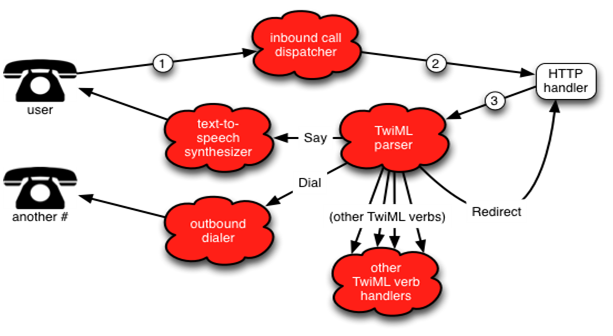
\includegraphics[width=\columnwidth]{image/Twilio-Architecture.PNG}
  \caption{Twilio Architecture~\cite{hid-sp18-406-twilio-architecture-image}}
\label{f:architecture}
\end{figure}


\subsection{Programmable Interfaces}

Twilio’s software-based platform provides developers with prefabricated building
blocks to integrate voice, messaging, video and several add-ons like sentimental
analysis into the application which are required to build communication 
functionality. These APIs are further developed as use case API’s which 
provide a higher level of abstraction of building communication interfaces for 
application and thus enabling programmable connectivity:
a. Authy: It is very important to authenticate the contact information when the 
user signs up into the business application. One of the best approaches is to do
account verification through SMS. Twilio provides two-factor authentication API.
By integrating this API, the application will be able to send the one-time 
password through text message and the user enters this code to complete the 
registration.  
b. Reminders: Automating the process of communicating with the customers using 
these Appointment Reminders API will help the customers to be updated about 
their appointment status. This API focuses on building appointment reminders 
when the appointment is created and until the time it is scheduled and attended.
c. Conference and Broadcast:
For any company to work collaboratively globally from various locations, it 
should be well organized to handle video conferences and broadcast abilities. 
Twilio provides APIs which enables any organization to build a moderate 
conference line that allows people to listen, speak or moderate during the call.
Voice Broadcasting APIs will allow broadcasting a pre-recorded voice message to 
a list of contacts.
d. Notifications:
In order to deliver time-sensitive alert messages, a text message is the most 
suitable way compared to emails as it helps to reach the end users quickly by 
avoiding the pile of inbox emails. APIs are provided to send out alert messages
as notifications from the web and mobile applications.
e. Click to Call
Customers always look for easy ways to reach their business people such as 
customer care. It is very important to keep the customers in such matters and 
Twilio provides Click to Call APIs for these requirements which enable 
developers to implement the call connections to the customer in the most 
suitable way.
f. Automated Survey
Feedback is an important factor which verifies the actual needs of customers and
the features which need to be improvised based on those requirements. Using the
Twilio’ automated survey APIs developer can build a survey form, which will
call the customer at the point of service to get immediate feedback opinions. 
Thus, these Automated Survey APIs integrates the customer relationship data to
the database without any difficulty.

Twilio’s scope is wide apart from the above-listed APIs including services for 
Masked Phone Numbers, Dynamic Call Center, Call Tracking, Call Forwarding, 
Workflow Automation, ETA Notifications, Instant Lead Alerts, Employee Directory
and many more~\cite{hid-sp18-406-twilio-architecture4}.
   
\section{Use case}
 
\subsection{General Usage}

The most basic use case of Twilio is to enable communication messages based on 
the scenarios. First, a developer will sign up for Twilio, then choose a local 
virtual number which is used to send and receive voice or SMS messages. The next
step is to map the virtual number to a request URL which will guide the 
communication interface how to manage the content of phone calls. Here, the 
developer will define a set of business rules or instructions to manage the 
calls from each customer. These rules include: 
a. Say – update the customer regarding the order update or play the prerecorded 
informational message 
b. Gather - collect all the required information from the user 
c. Record – record the complete call conversation 
d. Reject – Hang up 
e. Dial – make  a call to the number
Here, Twilio initiates the phone call or message flow on the one end and on the 
other end, it provides APIs for developers who will instruct or code the 
Twilio’s actions for those calls. Twilio also provides load balancing of the 
calls using cluster~\cite{hid-sp18-406-twilio-usecase1}.

\subsection{Communication for on-demand service}

Lyft is a ridesharing application. Its on-demand service requested by the 
customers requires real-time communication between the passengers and the 
drivers. By integrating Twilio communication APIs Lyft has ensured real-time 
SMS driver updates for passengers and also the ability of passenger calling the
driver without sharing the individual numbers. Here, when the ride is accepted 
by the driver, a communication channel is established without the dependency of
sharing the individual numbers. The call button on the application will 
initiate a phone call to the Twilio phone number assigned to that ride and 
routes to the driver’s mobile phone. Thus ensuring privacy standards for both
drivers and passengers. Lyft also uses other features of Twilio such as sending
notifications regarding the ride updates using the SMS integration API.  
Twilio’s unique feature such as masked numbers integrated for Lyft’s Lost and 
found procedure~\cite{hid-sp18-406-twilio-usecase1}.

Figure~\ref{f:usecase} explains the usecase of Twilio.


\begin{figure}[!ht]
  \centering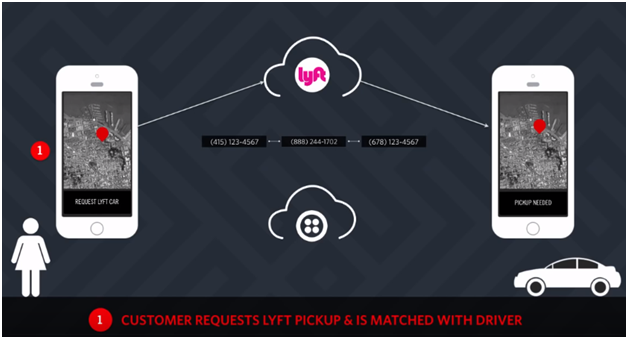
\includegraphics[width=\columnwidth]{image/Twilio-Usecase.PNG}
  \caption{Twilio Usecase~\cite{hid-sp18-406-twilio-usecase-image}}
\label{f:usecase}
\end{figure}



\section{Conclusion}
Twilio is basically a software as a service platform which provides a set of 
APIs which is hosted in the cloud and enables any developer to embed telephony 
into applications. Through its innovative ideas which target the daily needs of 
the customers, services provided by Twilio is increasing rapidly. With Twilio, 
you can reach customers in the ways they prefer, and engage with them 
effectively using context related to that interaction. As customer experience 
has become the significant factor, programmable communications have become more 
crucial than ever to the success of businesses today
~\cite{hid-sp18-406-twilio-conclusion1}. 

Twilio's customizable alerts help companies to determine the most suitable way 
to reach the users based on their preferences. Twilio has also extended APIs 
which allow developers to embed video conferencing within an application. Twilio
best fits the customer needs because of its global compatibility feature which 
includes more than 1000 wireless carriers around the world. By integrating  
telephony system into the application any business can establish an excellent 
way of extending use and authenticity for their IT solution. This helps the 
business to improve productivity, usability, reliability and perform the 
business in a cost-effective way. Hence, by mixing cloud and on-premises with 
mobile, Twilio enables developers to work on next-generation business tools
~\cite{hid-sp18-406-twilio-conclusion2}.

\begin{acks}

  The authors would like to thank Dr.~Gregor~von~Laszewski for his
  support and suggestions to write this paper.

\end{acks}

\bibliographystyle{ACM-Reference-Format}
\bibliography{report} 


